%!Tex root = bare_conf.tex

% 일반적으로, implementation은 algorithm 뒤에 오는 경우가 많음.
\section{Method}

\begin{figure}
\begin{subfigure}[b]{0.95\columnwidth}
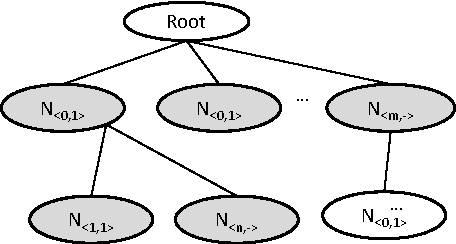
\includegraphics [width=0.95\columnwidth]{figures/sub_guess_1.pdf}
\caption{MCST with deciding whether to proceed with the game }
\label{fig:proceed_game}
\end{subfigure}
\par\bigskip
\begin{subfigure}[b]{0.95\columnwidth}
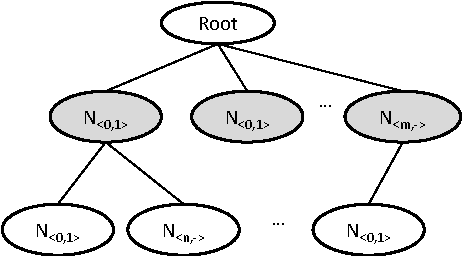
\includegraphics [width=0.95\columnwidth]{figures/sub_guess_2.pdf}
\caption{MCST with only stop choice}
\label{fig:stop_game}
\end{subfigure}
\caption{Simplification: not to keep guessing}
\end{figure}


We implemented two versions of MCTS for Da Vinci code. 
Firstly, we implemented the MCTS algorithm for Da vinci code (\cpu) which is running upon CPU environment.
We used OpenMP to parallelize the algorithm.
Secondly, we implemented the same algorithm which is running upon GPU environment (\gpu).
We used cuda to implement and parallelize the algorithm.

% Both versions are implemented in parallel. 
In the remaining of this section, we describes each version of algorithm in detail. 
As we modified the algorithm due to compuation overhead, we explain the algorithm design considerations compared to the vanilla version of MCTS.

\subsection{Designing Simplified Algorithm}

We designed the tree that each node represents the guessing tile's postion and guessing number.
% The \cref{fig:base_tree} shows the overall of MCTS for Da Vinci Code. 
Each node has position and number which are values that a player guesses.
Inherently, depth of tree means the number of guessing until the node.
As players in Da Vinci Code game do not know about other player's tile number, all simulations must be done in black-box manner.
We solve this problem by calculating plausible numbers of opponents tiles.
In each simulation, we randomly picked a set of plausible numbers of the tils, and conducted a simulation according to the numbers.
In this case, the same guessings (e.g., 5 to the leftmost tile) may induce the different results in the different simulation.
Therefore, a node must have information of the set of number to differentiate the results.
We treated this algorithm as a vanilla Da Vinci Code algorithm (\md).

% We implement simplified algorithm to reduce computation and proceed on real time, since original Da Vinci code has a lot of sibling nodes and child nodes which require a huge amount of computation and time limitation. 


We modified three parts of \md~to simplify the problem.
Firstly, we ignored a set of plausible numbers in view of node.
When we consider a set of plausible numbers, the number of child nodes is exploded.
For example, at the first turn, the root node can have at least 11880 number of chiled nodes.
We compute the number conservatively by considering the case that the opponent have the same colored four tiles.
Though the number is minimum of the number of cases, the number is much higher than 361, the number of go's.
We decided to ignore the set of plausible numbers, and only think of guessing position and guessing number because too many child nodes harm the quality of decision.
By ignoring the plausible set, we decreased the number of cases up to 88.

Secondly, we prohibited consecutive guessing.
A player who corrects the tile has chance to keep guessing or stop.
Therefore, \md has different player's node in the same depth~\cref{fig:proceed_game}.
The gray nodes mean that the same player keeps geussing.
This consecutive guessing makes the tree much complex, so we simplified this part.
We implemented Da Vinci code to always stop guessing when the player corrects the tile~\cref{fig:stop_game}.
To eliminating complex child node set, we could implement both of \cpu~and \gpu.
% Since original Da vinci code has numerous child node which make the decision tree unbalanced, we decided to implemente simple Da Vinci code which only has stop behavior.
 
\begin{figure}
\begin{subfigure}[b]{0.95\columnwidth}
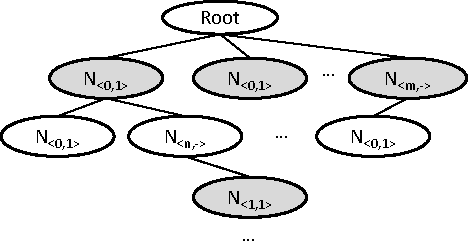
\includegraphics [width=0.95\columnwidth]{figures/sub_compare_expansion_1.pdf}
\caption{MCST with unlimited expansion}
\label{fig:expansion}
\end{subfigure}
\par\bigskip
\begin{subfigure}[b]{0.95\columnwidth}
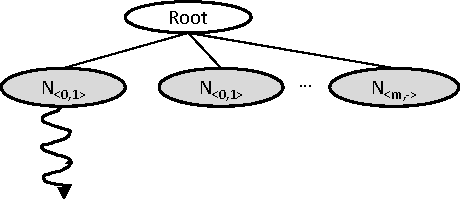
\includegraphics [width=0.95\columnwidth]{figures/sub_compare_expansion_2.pdf}
\caption{MCST with limited expansion}
\label{fig:limited_expansion}
\end{subfigure}
\caption{Simplification: limited expansion}
\end{figure}

Lastly, we limited the depth of expansion. 
Because Da Vinci Code has unlimited number of guessing in case of failing to guess, theoretical depth of tree is infinite.
This unrealistic cases can harm the performance of MCTS, so we fixed the depth of tree.
Nodes that has depth of the threshold conduct simulation and backpropagation, except expansion.
% 000000 on each depth, the number of cases makes a number of sibling nodes too hard to compute decision through MCTS. 
% In addition, too many cases make wrong decision, because root node has nodes that have similar winning rate. 
% Therefore, MCTS which we implemented has limitation of expansion. 
The \cref{fig:expansion} and \cref{fig:limited_expansion} show the difference bewteen original MCTS and simplified MCTS which we implemented.
By setting the expansion threshold as 1, we eliminates the unrealistic-depth node.
% We make one expansion from root and then the remaining turns are proceeded randomly. 
% The result of game updates expanded node from root and the MCTS doesn't make other expansion from frist depth. 


\begin{figure}
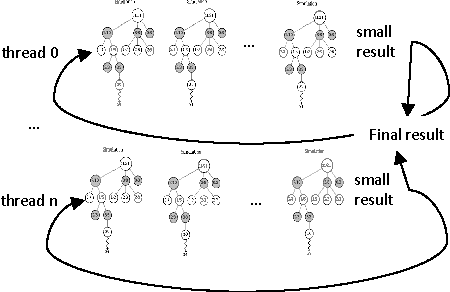
\includegraphics[width=0.95\columnwidth]{figures/implementation.pdf}
\caption{Overall process of creating MCTS}
\label{fig:implementation}
\end{figure}

\subsection{Implementation overview}
In MCTS implementation, each thread executes four stpes of MCTS repeatedly.
At this time, MCTS is conducted based on current state of a player and the oppenent.
Through simulating plays within a thread, a simulation makes small MCTS.
Each game in a thread expands the child node from root.
After the expansion, the game proceeds randomly. 
The result of simulation is updated to from the expanded node to the root node.
% The next game also expands the child node from the root and update the result of game to expanded node (depth one).
Each tread repeats this routine to generates results. 
The threads have small trees which are from simulation and these trees are combined to final MCTS.
Then, the player makes the decision based on the final MCTS.
The \cref{fig:implementation} shows the overall process how the MCTS is conducted.
% When the player comes to the turn, threads make final MCTS based on current state of the player and the oppenent. 
% The player makes the decision based on the final MCTS. 

\begin{itemize}
\item{Implementation of \textbf{\cpu}}\\
MCTS needs many simulated play repeatly to make good decision. 
% Parallelism can make MCTS construct good decision tree in a short period due to computating simultaneously.
MCTS based on CPU is implemented by openMP to utilize parallelism. 
Each thread computes simulations and derives a result(win or lose). 
After finishing derivation of result, all results from each thread are combined one MCTS.

\item{Implementation of \textbf{\gpu}}\\
% As we mentioned, MCTS needs parallelism to compute many cases for good decision. 
In GPU version, we use CUDA for paraller computation. 
Each tread computes simulations and derives a result(win or lose) as same as CPU version. 
After finishing deduction of result for each small MCTS, the small MCTS are combined final MCTS. 

\end{itemize}